\section{Experiments}

We used the Expectation-Maximization (EM) estimator and Method of Moments (MOM) estimator to estimate the parameters of the discrete mixture of models described in Section \ref{introduction}. We compare the estimators with the CRLB derived in Section 2.

The parameters in our model are $\alpha$, $p$, and $q$. We generated data using fixed values for these parameters, and then ran the estimators to find the values for these parameters. 
We applied the process for $p=0.2$, $q=0.4$, and for $\alpha=0.1, 0.2, \cdots, 0.9$. 
We set the length of each sequence to be $n=20$, and generated $N=200$ i.i.d. sequences.
We ran 200 independent Monte-Carlo runs.
We ran the EM algorithm for 100 iterations.

We compare the mean squared error (MSE) of each estimator and compare it to the CRLB.
The results are shown in Figure \ref{figure:crlb-em-mom}. 
As can be seen, the estimators have a bigger MSE when $\alpha=0.1$ or $\alpha=0.9$. 
This is because with $\alpha=0.1$, the data generator obtained sequences from the distribution $P(k_i(i)|p,n)$ with small probability.
The same happens when $\alpha=0.9$, where the data generator obtained sequences from the distribution $P(k_i(i)|q,n)$ with small probability.
The higher the probability that the data generator obtained sequences from a distribution, the easier it is for the estimators to estimate the correct value.
The performance of EM and MOM estimators is very similar, with differences mainly with small and large values for $\alpha$.

As can be seen, the CRLB is very low, compared to both estimators. 
To visualize the difference more clearly, we plotted the same results with a log-scale on the $y$ axis. 
The results are shown in Figure \ref{figure:crlb-em-mom-logscale}.
As can be seen, the CRLB is always more than 2 orders of magnitude lower than the results obtained by the estimators. 
We believe this is because the CRLB is not a tight bound. 
Therefore, in this case, the results obtained by the estimators do not get close to the CRLB.

\begin{figure}[!htbp]
	\centering
	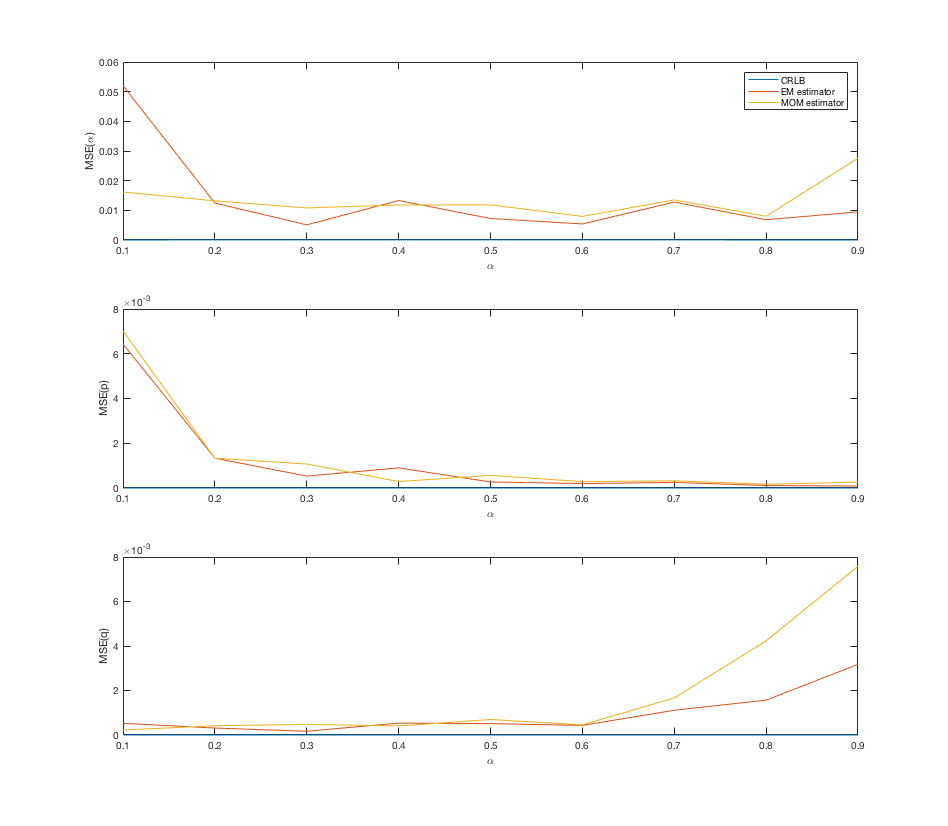
\includegraphics[width=\columnwidth]{images/CRLB_EM_MOM.png}
	\caption{CRLB, EM and MOM results for estimating $\alpha$ (top), $p$, (middle) and $q$ (bottom).}
	\label{figure:crlb-em-mom}
\end{figure}

\begin{figure}[!htbp]
	\centering
	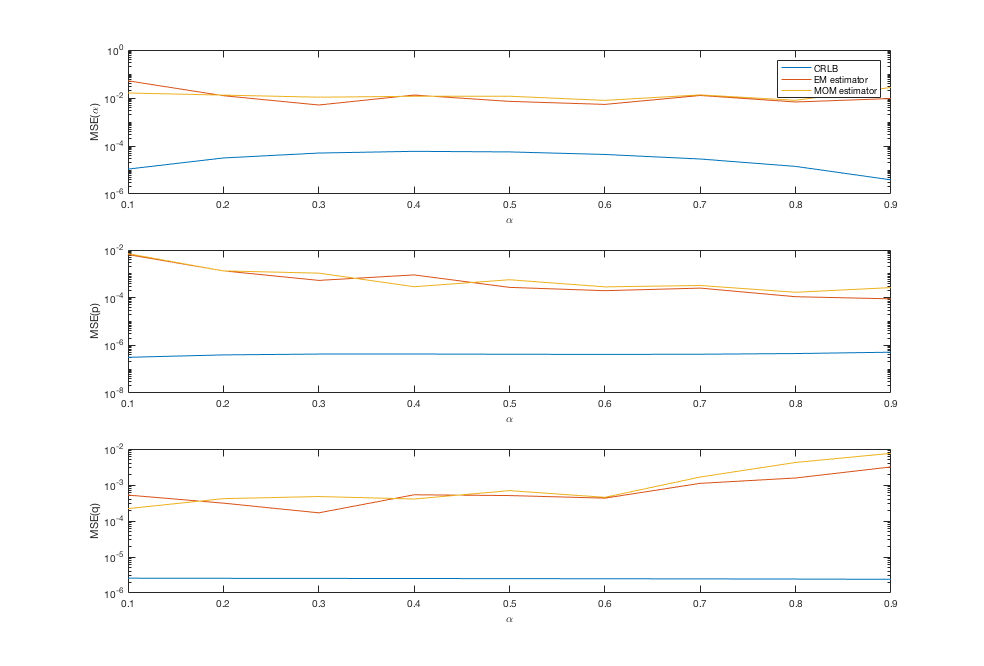
\includegraphics[width=\columnwidth]{images/CRLB_EM_MOM_log.png}
	\caption{CRLB, EM and MOM results for estimating $\alpha$ (top), $p$, (middle) and $q$ (bottom) with log-scale on the $y$ axis.}
	\label{figure:crlb-em-mom-logscale}
\end{figure}

\subsection{EM Initialization}

The performance of the EM algorithm may be affected by the initialization of the parameters. 
To evaluate the impact of initialization, we experimented with three methods of initialization.
The first method consists in setting initial values by selecting a random value from a uniform distribution between 0 and 1. This is the easiest method. However, the estimator may get stuck in a local minima.
In the second method, we use K-means clustering \cite{DBLP:journals/corr/BlomerB13}. This is a more informed method of initialization, without requiring much computational cost.
For the third method, we set the initial values to be the exact values that we used to generate the data. Although this is not reasonable in a practical sense, we consider this to be an ``empirical lower bound".
The results of running the EM algorithm with the described initialization methods are shown in Figure \ref{figure:em-init}. 
As can be seen, random initialization performs worse when $\alpha$ is low. 
However, it reaches a similar performance as other initialization methods with greater values of $\alpha$. 
K-Means initialization helps the estimator to obtain a lower MSE and get closer to our empirical lower bound.


\begin{figure}[!htbp]
	\centering
	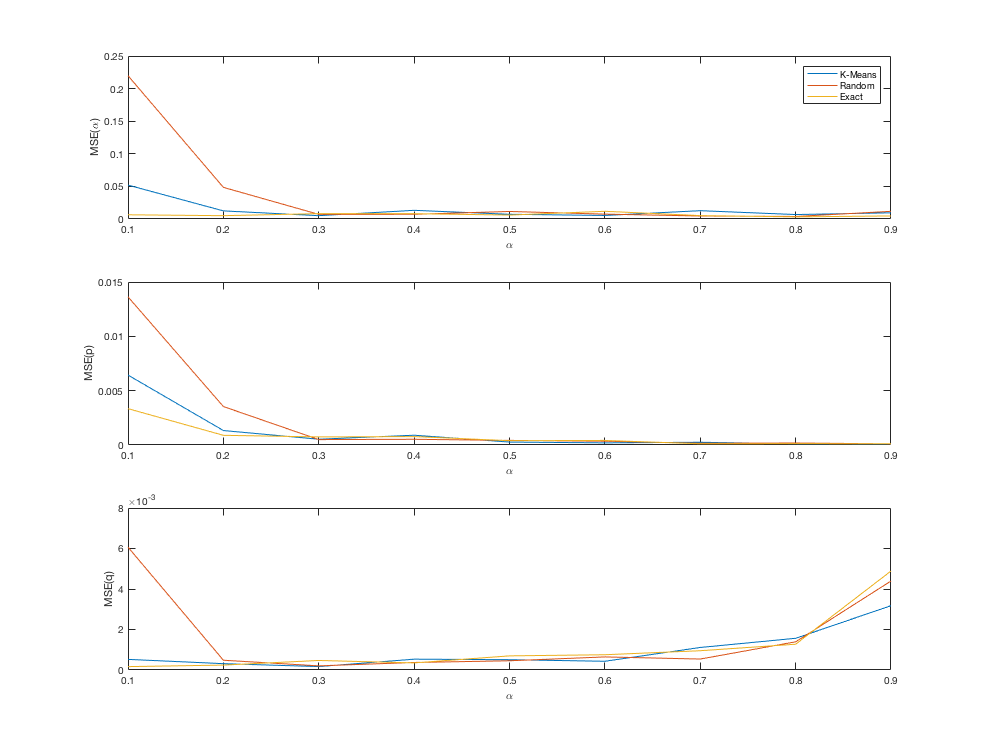
\includegraphics[width=\columnwidth]{images/compare_EM_init.png}
	\caption{EM results with different initializations for estimating $\alpha$ (top), $p$, (middle) and $q$ (bottom).}
	\label{figure:em-init}
\end{figure}

